\section{Вещественные числа}
    \subsection{Натуральные числа. Аксиоматика Пеано}
        \begin{definition} (Аксиоматика Пеано)
            \begin{enumerate}
                \item В множестве $\N$ $\forall n\in \N$ существует единственный элемент, называемый следующим и обозначаемый как $S(n)$.
                \item В множестве $\N$ $\forall n\in \N$ существует не более одного элемента, для которого $n$ - следующий.
                \item В множестве $\N$ существует единственный элемент $\N$, не являющийся следующим ни для какого элемента. Этот элемент обозначается $1$ и называется единицей.
                \item (Аксиома индукции) Пусть $M\subset \N$ такое, что $1\in M$ и $\forall m\in M:\\ S(m)\in M$. Тогда $M=\N$.
            \end{enumerate}
        Множество, удовлетворяющее этим аксиомам, называется множеством натуральных чисел и обозначается $\N$.
        \end{definition}
        \begin{definition}
            Рассмотрим  множество $X$. Если для некоторого $n\in \N$ существует биекция $\phi: X\to \{1, \dots n\}$, то $X$ называется $n$-элементным, или говорят, что количество элементов в $X$ равно $n$. Тот факт, что множество $X$ - $n$-элементное, обозначается как $|X|=n$ или $cardX=n$.
        \end{definition} 
        \begin{comm}
            По определению считаем, что $card(\emptyset) =0$.
        \end{comm}
        \begin{definition}
            Все множества, количество элементов которых равно какому-то натуральному числу или нулю, называются конечными. Все остальные множетсва называются бесконечными.
        \end{definition}
    \subsection{Отношение порядка и принцип наименьшего элемента}
        \begin{definition}
            $R\subset X\times Y$ называется отношением между элементами\\ $X$ и $Y$. Обозначают $xRy$, если $(x,y)\in R$.
        \end{definition}
        \begin{definition}
            Отношение $R$ называется отношением (линейного) порядка на множестве $X$, если $\forall x,y,z\in X$ выполнено:
            \begin{enumerate}
                \item $xRy$ или $yRx$. 
                \item $(xRy$ и $yRx) \Rightarrow x=y$. 
                \item $(xRy$ и $yRz) \Rightarrow xRz$.
            \end{enumerate}
            Такое отношение обозначают $\leq$.
        \end{definition}
        \begin{theorem}
            Существует единственное отношение порядка на $\N$ такое, что\\
            $\forall n\in \N: n\leq S(n)$.
        \end{theorem}
        \begin{proof}
            Без доказательства.
        \end{proof} 
        \begin{theorem} (Принцип наименьшего элемента)\\
            $M\subset \N, M\ne \emptyset$ имеет наименьший элемент, т.е. $\exists n_{min}\in M, \forall n\in M: n_{min}\leq n$.
        \end{theorem} 
        \begin{proof}
            Предположим, что в $M$ нет минимального элемента.\\
            База: если $1\in M$, то $n_{min}=1 \Rightarrow 1\notin M \Rightarrow 1\in \N\setminus M$.\\
            Шаг: $\{1,2,\dots, n\}\subset \N\setminus M \Rightarrow S(n)\in \N\setminus M$, тогда по аксиоме индукции $\N\setminus M=\N\Rightarrow M = \emptyset$ - противоречие.
        \end{proof}
    \subsection{Арифметические операции}
        \begin{definition}
            Рассмотрим множества $A$ и $B, card(A)=n, card(B)=k,\\
            n,k\in \N$. Пусть $A\cap B=\emptyset$. Тогда число $card(A\cup B)$ называется суммой $n$ и $k$ и обозначается $card(A\cup B)=n+k$.
        \end{definition}
        \begin{comm}
            Естественно выполняется $n+k=k+n$ (коммутативность) и\\ $(n+k)+m=n+(k+m)$ (ассоциативность).
        \end{comm}
        \begin{comm}
            $n+0=0+n=n$, т.к. $cardA=card(A\cup \emptyset)$.
        \end{comm}
        \begin{comm}
            По определению существуют биекции $A \leftrightarrow \{1,\dots, n\}, B\leftrightarrow \{1,\dots, k\}$. Возьмем $card(A\cup B)=\{1,\dots, n\}\cup \{\underbrace{S(n), S(S(n)), \dots, S(S(\dots (S(n))\dots)}_k\}$,\\ (где $\{1,\dots, k\} \leftrightarrow \{\underbrace{S(n), S(S(n)), \dots, S(S(\dots (S(n))\dots)}_k\})$\\
            Из тех же соображений получаем, что $S(n)=n+1$.
        \end{comm} 
        \begin{definition}
            $n,k\in \N$. Тогда $\sum\limits_{i=1}^kn=nk$ называется произведением $n$ на $k$.
        \end{definition}
        \begin{comm} Выполнены:
            \begin{itemize}
                \item $nk=kn$ (коммутативность)
                \item $n(km)=(nk)m$ (ассоциативность)
                \item $k(n+m)=kn+km$ (дистрибутивность)
                \item Если $k\leq n$, то $k+m\leq n+m$ и если $k\leq m$, то $kn\leq mn$
            \end{itemize}
        \end{comm}
        \begin{definition}
            Если $n+k=m$, то $n=m-k$ называется разностью\\ $m$ и $k,\ k=m-n$ называется разностью $m$ и $n$.
        \end{definition}
        \begin{comm}
            $m-0=m,\ m+0=m,\ m-m=0$.
        \end{comm}
        \begin{definition}
            $nk=m, \frac{m}{n}=k, \frac{m}{k}=n$.
        \end{definition}
    \subsection{Целые числа}
        \begin{definition}
            Введем набор символов $-\N=\{\dots,-2,-1\}$. Множество символов $-\N \cup\{0\}\cup \N$ называется целыми числами и обозначаются $\Z$. 
            В нем принимаем выполненными следующие свойства:
            \begin{enumerate}
                \item $k+(-n)=\begin{cases}
                    k-n, \text{если} \hspace*{5pt} k\geq n,\\
                    -(n-k), \text{если} \hspace*{5pt} k<n.
                \end{cases}$.\\
                $(-k)+(-n)=-(k+n)$
                \item $k\cdot 0= (-k)\cdot 0=0$,\\
                $(-k)\cdot n=(-kn)$,\\
                $(-k)(-n)=kn$.
                \item $(\pm k)((\pm n)+(\pm m))=(\pm k)(\pm n)+(\pm k)(\pm m)$.
                \item $\forall k: (-k)\leq 0,\\$
                $(-k)\leq (-n)$, если $n\leq k$.
                \item $\forall (\pm k), (\pm n), (\pm m)\in \Z$, если $(\pm k)\leq (\pm n)$, то $(\pm k)+(\pm m)\leq (\pm n)+(\pm m)$.
                \item $\forall (\pm n), (\pm k)\in \Z, m\in \N$, если $(\pm n)\leq (\pm k)$, то $(\pm n)m\leq (\pm k)m$.
            \end{enumerate}
        \end{definition}
        Далее пишем $-k$ вместо $(-k)$.\\
        $\forall k,n\in \Z$ $\exists (k-n)=k+(-n)$.
    \subsection{Рациональные числа}
        \begin{definition}
            Множество $\Q=\{(m,n)\in \Z \times \N\}$, элементы которого обозначают $\frac{m}{n}$ называется множеством рациональных чисел, если введены следующие операции:
            \[\frac{m}{n}+\frac{p}{q}=\frac{mq+pn}{nq}\]
            \[\frac{m}{n}\cdot \frac{p}{q}=\frac{mp}{nq}\]
            а также введено отношение порядка:
            \[\frac{m}{n}\leq \frac{p}{q}\ \Leftrightarrow\ mq\leq pn\]
        \end{definition}
        Свойства операций $(a,b,c \in \Q)$:
        \begin{enumerate}
            \item $a+b=b+a$
            \item $a+(b+c)=(a+b)+c$
            \item $\exists ! \hspace{5pt} 0 \in \Q: a+0=0+a=a$
            \item $\forall a\in \Q \hspace{5pt} \exists ! \hspace{5pt} (-a)\in \Q: a+(-a)=0$
            \item $ab=ba$
            \item $a(bc)=(ab)c$
            \item $\exists ! \hspace{5pt} 1\in \Q \hspace{5pt} \forall a: a\cdot 1=1\cdot a=a$
            \item $\forall a\ne 0 \hspace{5pt} \exists ! \hspace{5pt} a^{-1}: aa^{-1}=a^{-1}a=1$
            \item $a(b+c)=ab+ac$
            \item $\forall a,b\in \Q \hspace{5pt} a\leq b$ или $b\leq a$
            \item $a\leq b$ и $b\leq a \Rightarrow a=b$
            \item $a\leq b$ и $b\leq c \Rightarrow a\leq c$
            \item $\forall c \in \Q: a\leq b \Rightarrow a+c\leq b+c$
            \item $\forall c\in \Q: c>0: a\leq b\Rightarrow ac\leq bc$
        \end{enumerate}
    \subsection{Упорядоченные и архимедовы поля}    
        \begin{definition}
            Множество $X$ с операциями $(\cdot, +)$ и отношением порядка $\leq$ называется упорядоченным полем.
        \end{definition}
        \begin{comm}
            $\Q$ - упорядоченное поле.
        \end{comm}  
        \begin{definition}
            Упорядоченное поле $X$ называется архимедовым, если\\
            15.\ $\forall a\in X: \exists\ n\in \N: a\leq n$.
        \end{definition}
        \begin{comm}
            $\Q$ - архимедово поле.
        \end{comm} 
        \begin{comm}
            $\frac{m}{n}=\frac{p}{q} \Leftrightarrow mq=pn$.
        \end{comm}
        \begin{comm}
            $\forall m\in \Z$ число $\frac{m}{1}\in \Q$ можно отождествить с $m$.
        \end{comm}
    \subsection{Действительные числа. Аксиома полноты}
        \begin{definition}
            Множество $\R$ называется множеством действительных чисел, если $\Q \subset \R$, $\R$ удовлетворяет (1)-(15) и дополнительно выполняется (16).
        \end{definition}
        \begin{axiom} (Аксиома полноты)\\
            16.\ $\forall A,B\subset \R$ таких, что $\forall a\in A,\ \forall b\in B: a\leq b \ \exists \ c\in \R: a\leq c\leq b$.
        \end{axiom}
        \begin{example}
        Аксиома полноты не выполняется в $\Q$.\\
        $A=\{a\leq 0$ или $a>0: a^2<2\}$, $B=\{b>a: b^2>2\}$,\\
        но не существует $\frac{m}{n}$ такого, что $\frac{m^2}{n^2}=2$
        \end{example}
    \subsection{Модели действительных чисел}
    \subsubsection*{Модель бесконечных десятичных дробей}
        \begin{definition}
            Отображение $\{a_n\}: \N \to X$ называется последовательностью элементов $X$.
        \end{definition}
        \begin{definition}
            Выражение вида $\pm a_0,a_1,\dots, a_n, \dots$ называется бесконечной десятичной дробью, если $a_0\in \N$ или $a_0=0$\ и $\forall i\in \N: a_i \in \{0,1,\dots, 9\}$.
        \end{definition}
        \begin{definition}
            Введем отношение порядка $\leq$ на множестве всех бесконечных десятичных дробей следующим образом:
            \begin{enumerate}
                \item Если $a_0\leq 0,$ $b_0>0$, то $a\leq b$.
                \item Если $a_0, b_0\geq 0,$ то $a\leq b$
                \begin{itemize}
                    \item если $a_0<b_0$ или $a_0=b_0$, $a_1<b_1$ или $a_0=b_0$, $a_1=b_1$, $a_2<b_2$,\\ или \dots или $a_0=b_0$, $a_1=b_1$, $a_2=b_2, \dots, a_{n-1}=b_{n-1},$ $a_n<b_n\dots$
                    \item если $a_0=b_0$, $a_1=b_1, \dots, a_{n-1}=b_{n-1}$, а также $a_n\ne 9, b_n=a_{n}+1$.
                    $a_{n+k}=9$, $b_{n+k}=0$, $\forall k \in \N$, т.е $a=\overline{a_0a_1...a_n(9)}$, а $b=\overline{b_0b_1...b_n(0)}$.\\
                    (в числе $a$ начиная с $a_{n+1}$ все $a_i$ равны 9, а в числе $b$ начиная с $b_{n+1}$ все $b_i$ равны 0), то $a=b$.
                \end{itemize}
                \item Если $a_0, b_0<0$, то $a\leq b$, если $-b\leq -a$ (случай 3 сведен к случаю 2)
            \end{enumerate}
        \end{definition} 
        \begin{theorem}
            Множество бесконечных десятичных дробей с введенным отношением порядка $(\leq)$ удовлетворяет аксиоме полноты.
        \end{theorem} 
        \begin{proof}
            Пусть $A,B\subset$ $\{$множество бесконечных десятичных дробей$\}$ и $\forall a\in A, \forall b\in B: a\leq b$.
            \begin{enumerate}
                \item $a<0, b\geq 0$, тогда $c=0$.
                \item $a\geq 0, b\geq 0$\\
                Пусть\\
                $\overline{b_0}=\min \{b_0: b_0b_1b_2\dots \in B\},\\
                \overline{b_1}=\min \{b_1: \overline{b_0}b_1b_2\dots \in B\}$,\\
                $\overline{b_2}=\min \{b_2: \overline{b_0}\overline{b_1}b_2 \dots \in B\}$,\\
                \vdots \\
                Возьмем $\overline{b}= \overline{b_0b_1b_2\dots b_n \dots}\in B$, тогда\\
                $\forall a\in A, \forall b\in B: a\leq \overline{b}\leq b$.\\
                \item $a<0, b<0$ строим число по аналогии с пунктом 2.
            \end{enumerate}
        \end{proof} 
    \subsubsection*{Дедекиндовы сечения}
        \begin{definition}
            Пусть $A,B\subset \Q: A\cap B = \emptyset,\ A\cup B=\Q,\ \forall a\in A,\ \forall b\in B:\\
            a\leq b$ и в $B$ не существует минимального элемента, тогда $(A,B)$ - пара сечений $\Q$.
        \end{definition} 
        \begin{theorem}
            На множестве всех пар сечений $\{(A,B)\}$ можно ввести операции $(+), (\cdot)$ и отношение $(\leq)$, так что будут выполняться $(1)-(16)$.
        \end{theorem} 
        \begin{proof}
            Без доказательства.
        \end{proof}
    \subsubsection*{Геометрическая модель числовой прямой}
    Выбираем точку, называем ее 0
    \[\begin{tikzpicture}
        \draw[-latex] (-5.5,0) -- (5.5,0) ;
        \foreach \x in  {0}
        \draw[shift={(\x,0)},color=black] (0pt,3pt) -- (0pt,-3pt);
        \foreach \x in {0}
        \draw[shift={(\x,0)},color=black] (0pt,0pt) -- (0pt,-3pt) node[below] 
        {$\x$};
        \end{tikzpicture}\]
        затем выбираем точку справа от него, называем ее 1
        \[\begin{tikzpicture}
        \draw[-latex] (-5.5,0) -- (5.5,0) ;
        \foreach \x in {0,1}
        \draw[shift={(\x,0)},color=black] (0pt,3pt) -- (0pt,-3pt);
        \foreach \x in {0,1}
        \draw[shift={(\x,0)},color=black] (0pt,0pt) -- (0pt,-3pt) node[below] 
        {$\x$};
        \end{tikzpicture}\]
        затем вводим сложение и получаем $2, 3, 4$, и т.д. (натуральный ряд)
        \[\begin{tikzpicture}
        \draw[-latex] (-5.5,0) -- (5.5,0) ;
        \foreach \x in {0,1,2,3,4}
        \draw[shift={(\x,0)},color=black] (0pt,3pt) -- (0pt,-3pt);
        \foreach \x in {0,1,2,3,4}
        \draw[shift={(\x,0)},color=black] (0pt,0pt) -- (0pt,-3pt) node[below] 
        {$\x$};
        \end{tikzpicture}\]
        затем делаем также в другую сторону, получаем целые числа
        \[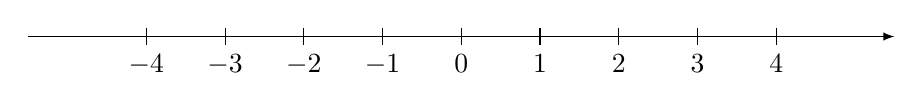
\begin{tikzpicture}
        \draw[-latex] (-5.5,0) -- (5.5,0) ;
        \foreach \x in {-4,-3,-2,-1,0,1,2,3,4}
        \draw[shift={(\x,0)},color=black] (0pt,3pt) -- (0pt,-3pt);
        \foreach \x in {-4,-3,-2,-1,0,1,2,3,4}
        \draw[shift={(\x,0)},color=black] (0pt,0pt) -- (0pt,-3pt) node[below] 
        {$\x$};
        \end{tikzpicture}\]
        Проведем через 0 под непрямым углом вспомогательную прямую на ней выберем точку, назовем ее $1^{\prime}$ и аналогично первой прямой получаем на ней целые числа. Проведем прямую через $n^{\prime}$ и 1 тогда параллельная ей прямая проходящая через $1^{\prime}$ проходит через $\frac{1}{n}$ (по теореме Фаллеса)
        \begin{figure}[h]
            \centering
            \includegraphics[width=0.8\linewidth]{Pictures/falles.png}
        \end{figure}\\
        таким образом складывая $m$ раз $\frac{1}{n}$, получим любое рациональное число $\frac{m}{n}$.\\
        Построим бесконечную десятичную дробь, например $0,37152\dots$.\\
        Разобьем отрезок:
        \[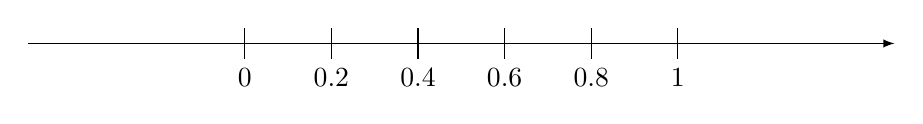
\begin{tikzpicture} [scale=5.5]
        \draw[-latex] (-0.5,0) -- (1.5,0) ;
        \foreach \x in {0,0.2,0.4,0.6,0.8,1}
        \draw[shift={(\x,0)},color=black] (0pt,1pt) -- (0pt,-1pt);
        \foreach \x in {0,0.2,0.4,0.6,0.8,1}
        \draw[shift={(\x,0)},color=black] (0pt,1pt) -- (0pt,-1pt) node[below] 
        {$\x$};
        \end{tikzpicture}\]
        $0,37152\dots$ находится между $0.2$ и $0.4$, теперь разобьем этот отрезок:
        \[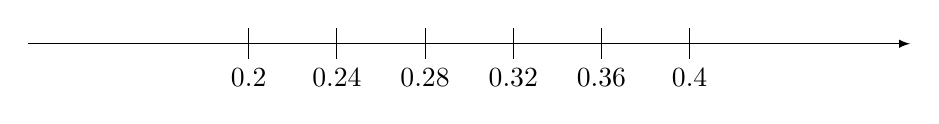
\begin{tikzpicture} [scale=28]
        \draw[-latex] (0.1,0) -- (0.5,0) ;
        \foreach \x in {0.2,0.24,0.28,0.32,0.36,0.4}
        \draw[shift={(\x,0)},color=black] (0pt,0.2pt) -- (0pt,0.2pt);
        \foreach \x in {0.2,0.24,0.28,0.32,0.36,0.4}
        \draw[shift={(\x,0)},color=black] (0pt,0.2pt) -- (0pt,-0.2pt) node[below] 
        {$\x$};
        \end{tikzpicture}\]
        $0,37152\dots$ находится между $0.36$ и $0.4$, теперь разобьем этот отрезок и т.д.
        Получаем последовательность вложенных отрезков, у которых длина стремится к нулю, значит у них есть единственная общая точка - наше число.\\
        Таким образом, прямая - множество бесконечных десятичных дробей, а значит на ней выполняеются (1)-(16).
        \subsection{Принципы полноты}
        %\subsubsection{Верхние и нижние грани множества}
        \begin{definition} \tab
            \begin{itemize}
                \item Элемент $a\in \R$ называется максимальным элементом множества $A$\\ $(\max A\subset \R), A\ne \emptyset$, если $\forall a^{\prime}\in A: a\geq a^{\prime}$ и $a\in A$.
                \item Элемент $a\in \R$ называется минимальным элементом множества $A$\\ $(\min A\subset \R), A\ne \emptyset$, если $\forall a^{\prime}\in A: a\leq a^{\prime}$ и $a\in A$.
            \end{itemize}
        \end{definition} \tab
        \begin{definition} \tab
            \begin{itemize}
                \item Элемент $m\in \R$ называется верхней гранью $A\subset \R, A\ne \emptyset$, если\\ $\forall a\in A: a\leq m$.
                \item Элемент $m\in \R$ называется нижней гранью $A\subset \R, A\ne \emptyset$, если\\ $\forall a\in A: a\geq m$.
            \end{itemize}
        \end{definition}
        \begin{definition} \tab
            \begin{itemize}
                \item Множество $A \subset \R, A\ne \emptyset$ называется ограниченным сверху, если у $A$ существует верхняя грань.
                \item Множество $A \subset \R, A\ne \emptyset$ называется ограниченным снизу, если у $A$ существует нижняя грань.
                \item Множество $A \subset \R$ называется ограниченным, если $A$ ограничено и сверху и снизу.
            \end{itemize}
        \end{definition}
        \begin{definition} \tab
            \begin{itemize}
                \item Пусть множество $A \subset \R$ ограничено сверху, $B$ - множество верхних граней $A$. Элемент $c=\min B$ называется точной верхней гранью $A$ и обозначается $\sup A$.
                \item Пусть множество $A \subset \R$ ограничено снизу, $B$ - множество нижних граней $A$. Элемент $c=\max B$ называется точной нижней гранью $A$ и обозначается $\inf A$.
            \end{itemize}
        \end{definition}
        %\subsubsection{Принцип полноты Вейерштрасса}
        \begin{theorem} (Принцип полноты Вейерштрасса) \\
            Для каждого ограниченого сверху или снизу множества $A$ существует $\sup A$ или $\inf A$ соответственно.
        \end{theorem}
        \begin{proof}
            Докажем для верхней грани (аналогично для нижней)\\
            $A$ - ограничено сверху, $B$ - множество верхних граней. Значит $\forall a\in A$ и \\$\forall b\in B: a\leq b \Rightarrow$ по аксиоме полноты $\exists\ c\in \R: a\leq c\leq b \Rightarrow c=\sup A$.
        \end{proof}
        \begin{lemma} (Свойство точной грани)\\
            Если у множества $A\subset \R$ существует $M=\sup{A}$ или $m=\inf{A}$, то $\forall \epsilon>0\ \exists\ a\in A: a\in (M-\epsilon,M)$ или $a\in (m,m+\epsilon)$ соответственно.
        \end{lemma}
        \begin{proof}
            Докажем для верхней грани. $M=\sup{A}\Rightarrow \forall a\in A: a\leq M$. Поскольку $M$ - минимальная из верхних граней, то $\forall \epsilon>0: \widetilde{M}=M-\epsilon$ - не является верхней гранью. Тогда $\exists\ a\in A: a>\widetilde{M} \Rightarrow a\in (M-\epsilon,M)$.
        \end{proof} 
        \begin{definition}
            $\forall a,b\in \R: a<b$ рассмотрим следующие множетсва:
            \begin{itemize}
                \item $[a,b] := \{x\in \R: a\leq x\leq b\}$ - отрезок
                \item $(a,b) := \{x\in \R: a<x<b\}$ - интервал
                \item $[a,b) := \{x\in \R: a\leq x<b\}$ - полуинтервал
                \item $(a,b] := \{x\in \R: a<x\leq b\}$ - полуинтервал
            \end{itemize}
            Такие множества называют промежутками.
        \end{definition} 
        \begin{definition}
            $\forall a\in \R$ функция
            \[|a|=
                \begin{cases}
                    \tab[12pt]a, \tab[5pt] a\geq 0,\\
                    -a, \tab[5pt] a<0.
                \end{cases}\]
            называется модулем.
        \end{definition}
        \begin{definition}
            Для любого промежутка с концами $a,b\in \R$ длиной называется число $|b-a|$.
        \end{definition}
        \begin{definition}
            Рассмотрим последовательность $\{[a_n,b_n]\}_{n=1}^{\infty}$. Говорят, что\\ $|b_n-a_n|\to 0$ при $n\to \infty$, если $\forall \epsilon >0\tab[5pt]\exists N\in \N: \forall n>N$ выполнено $|b_n-a_n|<\epsilon$.
        \end{definition}
        %\subsubsection{Принцип вложенных отрезков (принцип полноты Кантора)}
        \begin{theorem} (Принцип вложенных отрезков, принцип полноты Кантора) \\
            Пусть последовательность $\{[a_n,b_n]\}_{n=1}^{\infty}$ такова, что $\forall n: [a_{n+1},b_{n+1}]\subset [a_n,b_n]$. Тогда $\exists\ c\in \R: c\in [a_n,b_n], \forall n$. Если $|b_n-a_n|\to 0$ то $c$ - единственная.
        \end{theorem} 
        \begin{proof}
            $\forall n,m\in \N: a_n\leq b_m$, т.к
            \begin{itemize}
                \item если $n<m$, то $a_n\leq a_m\leq b_m$.
                \item если $n>m$, то $a_n\leq b_n\leq b_m$.
            \end{itemize}
            Значит для $\forall m,n\in \N: $
            Рассмотрим множества $A=\{a_n\}$ и $B=\{b_n\}$. По аксиоме полноты $\exists\ c\in \R: a_n\leq c\leq b_m,\ \forall n,m \Rightarrow a_n\leq c\leq b_n,\ \forall n$.\\
            Пусть $|b_n-a_n|\to 0$, предположим, что $\exists\ c_1$ и $c_2: c_1\ne c_2$ - различные общие точки, значит $|c_2-c_1|>0$. Получаем, что $0<|c_2-c_1|<|b_n-a_n|,\ \forall n$, значит $|c_2-c_1|\to 0$ получаем противоречие.
        \end{proof} 
        \subsection{Отношение эквивалентности. Равномощные множества}
        \begin{definition}
            Отношение $\sim$ называется отношением эквивалентности, если оно удовлетворяет:
            \begin{enumerate}
                \item $x\sim x$ (Рефлексивность)
                \item $x\sim y \Rightarrow y\sim x$ (Симметричность)
                \item $x\sim y$ и $y\sim z\Rightarrow x\sim z$ (Транзитивность)
            \end{enumerate}
        \end{definition} 
        \begin{definition}
            Множества называются равномощными, если между ними существует биекция.
        \end{definition}
        \begin{theorem}
            Равномощность множеств является отношением эквивалентности.
        \end{theorem}
        \begin{proof} Пусть $A,B,C$ - множества, $\phi:A\to B, \psi:B\to C$ - биекции.
            \begin{enumerate}
                \item Рефлексивность очевидна, поскольку у любого множества существует биекция в себя.
                \item Для любой биекции $\phi:A\to B$ существует $\phi^{-1}:B\to A$.
                \item $\phi:A\to B,\ \psi:B\to C$, то $\psi \circ \phi: A\to C$.
            \end{enumerate}
        \end{proof} 
        \begin{comm}
            Если $A$ равномощно $B$ то иногда пишут $A\sim B$ или $|A|=|B|$.
        \end{comm} 
        \begin{theorem}
            Конечные множества равномощны $\Leftrightarrow$ они содержат одинаковое количество элементов.
        \end{theorem}
        \begin{proof}\tab
            \begin{itemize}
                \item[$(\Leftarrow)$] Пусть $\phi:A\to \{1,\dots, n\}, \ \psi:B\to \{1,\dots, n\}\\
                \Rightarrow \exists \ \psi^{-1}:\{1,\dots, n\}\to B$. Тогда $\phi \circ \psi^{-1}:A\to B$ - искомая биекция.
                \item[$(\Rightarrow)$] Пусть $\phi:A\to B$ - биекция, если $A=\emptyset$, то $B=\emptyset$. Индукция по количеству элементов. База: пусть $A=\{a\}$, тогда $\exists ! \ b\in B: \phi(a)=b$. Пусть утверждение верно для случая когда $A$ - это $n$-элементное множество. Теперь если $A$ - это $n+1$-элементное, то $\exists \ \phi:A\to \{1,2,...,n+1\}$ - биекция. Значит $\exists ! \ a\in A$, что $\phi(a)=n+1$. Тогда $A\setminus\{a\}$ - $n$-элементное и $\exists ! \ b\in B: b=\phi(a) \Rightarrow B\setminus\{b\}$ - $n$-элементное $\Rightarrow  B$ - $n+1$-элементное.
            \end{itemize}
        \end{proof}
        \begin{definition}
            Множества, равномощные $\N$ называются счетными.
        \end{definition} 
        \begin{definition}
            Множество называется не более чем счетным, если оно конечно или счетно.
        \end{definition}
        \begin{theorem}
            Объединение не более чем счетного числа счетных множеств счетно.
        \end{theorem}
        \begin{proof}
            Предъявим проход по элементам, который задает биекцию:
            \begin{center}
                \includegraphics[width=0.4\linewidth]{Pictures/prohod.png}
            \end{center}
        \end{proof}
        \begin{consequense}
            Объединение не более чем счетного числа не более чем счетных множеств не более чем счетно.
        \end{consequense} 
        \begin{examples}\tab
            \begin{enumerate}
                \item Множество целых чисел $\Z$ счетно.
                \item Множество рациональных чисел $\Q$ счетно.
                \item Множество многочленов с рациональными коэффициентами счетно.
                \item Множество алгебраических чисел (чисел которые являются корнями многочлена с рациональными коэффициентами) счетно.
            \end{enumerate}
        \end{examples}
        \subsection{Теорема Кантора и аксиома выбора}
        % \begin{theorem} (Теорема Кантора)\\
        %    Множество бесконечных последовательностей, состоящих из нулей и единиц несчетно.
        % \end{theorem} 
        % \begin{proof}
        %    Предположим, что оно счетно. Тогда все последовательности нулей и единиц можно перенумеровать. Составим бесконечную вниз таблицу, строками которой будут наши последовательности:\\
        %    \tab[6cm]$a_1=\underline{a_{11}}\ a_{12}\ a_{13}\ a_{14}\ \dots$\\
        %    \tab[6cm]$a_2=a_{21}\ \underline{a_{22}}\ a_{23}\ a_{24}\ \dots$\\
        %    \tab[6cm]$a_3=a_{31}\ a_{32}\ \underline{a_{33}}\ a_{34}\ \dots$\\
        %    \tab[6cm]$a_4=a_{41}\ a_{42}\ a_{43}\ \underline{a_{44}}\ \dots$\\
        %    \tab[6cm]\vdots\\
        %    $a_{ij}$ - $j$-й член $i$-й последовательности. Рассмотрим последовательность $b$ у которой $b_i=1-a_{ii}$. Такая последовательность отличается от каждой $i$-й последовательности на $i$-й позицции, значит она не была посчитана, получаем противоречие.
        % \end{proof}
        \begin{theorem} (Теорема Кантора)\\
            Интервал $(0,1)$ несчетен.
        \end{theorem}
        \begin{proof}\footnote{Может немного отличаться от доказательства на лекциях}
            Докажем от противного. Предположим, что у нас получилось перечислить все элементы интервала $(0,1)$ 
            \[x_1=0,\ a_{11}\ a_{12}\ a_{13}\ \dots\]
            \[x_2=0,\ a_{21}\ a_{22}\ a_{23}\ \dots\]
            \[x_3=0,\ a_{31}\ a_{32}\ a_{33}\ \dots\]
            \[\vdots\]
            \newpage
            Теперь построим такую последовательность $b$, задающую число, которого нет в списке. Определим последовательность так: $b_0 = 0$ и на $i$-й позиции $b_i$ отличается от $a_{ii}$, например зададим ее так:
            \[b_i=
            \begin{cases}
                1,\ \text{если},\ a_{ii}\ne 1,\\
                2,\ \text{если},\ a_{ii}=1.
            \end{cases}\]
            Таким образом, построенное число $x = 0,\ b_1\ b_2\ b_3\ \dots$ отличается от каждого из $x_1,x_2,x_3\dots$ на $i$ позиции $\Rightarrow$ оно не было пересчитано, получаем противоречие.
        \end{proof} 
        \begin{consequense}
            Действительных чисел несчетно.
        \end{consequense} 
        \begin{proof}\footnote{Не было на лекциях}
            Достаточно показать, что $\R \sim (0,1)$. Например функция\\
            $f:(0,1)\to \R$, такая что $f(x)=\frac{2x-1}{4x-4x^2}$ задает нужную биекцию.
        \end{proof} 
        \begin{definition}
            Действительные числа не являющиеся алгебраическими называются трансцендентными.
        \end{definition} 
        \begin{definition}
            Множества равномощные интервалу $(0,1)$ называются множествами мощности континуума.
        \end{definition} 
        \begin{theorem}
            У любого множетсва мощность множества всех подмножеств строго больше чем мощность самого множества.
        \end{theorem}
        \begin{proof}
            Без доказательства.
        \end{proof} 
        \begin{definition}
            Для множеств $A$ и $B$ обозначим $|A|\leq |B|$, если $\exists \ B^{\prime} \subset B$ такое, что $A\sim B^{\prime}$.
        \end{definition} 
        \begin{theorem}
            Сравнение мощностей множеств $|A|\leq |B|$ является отношением порядка.
            \begin{enumerate}
                \item $\forall A,B: |A|\leq |B|$ или $|B|\leq |A|$ 
                \item $|A|\leq |B|$ и $|B|\leq |A| \Rightarrow |A|=|B|$\ (Теорема Кантора-Бернштейна)
                \item $|A|\leq |B|$ и $|B|\leq |C| \Rightarrow |A|\leq |C|$
            \end{enumerate}
        \end{theorem}
        \begin{proof}
            Без доказательства.
        \end{proof}
        \begin{axiom}(Аксиома выбора)\\
            Если существует семейство непустых множеств, то из каждого множества можно выбрать по одному элементу и составить из них другое множество.
        \end{axiom}
        \begin{statement}
            Множество $2^{\N}$ всех подмножеств $\N$ равномощно интервалу (0,1) (множеству $\{0,1\}^{\N}$ бесконечных последовательностей нулей и единиц).
        \end{statement}
        \begin{proof}\footnote{Может отличаться от доказательства на лекциях}
            Каждому $A\subset \N$ ставим в соответствие характеристическую последовательность, которая принимает значения: единицу, если элемент лежит в подмножестве и ноль иначе $\Rightarrow 2^{\N}\sim \{0,1\}^{\N}$. Поскольку каждое число из интервала $(0,1)$ представляется как последовательность цифр $0,\ a_1,\ a_2,\ a_3,\ \dots$ и каждую цифру можно представить в двоичной системе исчисления, то можно сделать вывод, что $2^{\N}\sim (0,1)$.
        \end{proof}
        \begin{theorem}
            У любого бесконечного множества существует счетное подмножество.
        \end{theorem} 
        \begin{proof}
            Выбираем элемент и сразу присваиваем ему номер. Продолжая это действие, построим счетное множество.
        \end{proof}
        \begin{theorem}
            Пусть $A$ - бесконечное, $B$ - не более чем счетное $\Rightarrow A\sim A\cup B$
        \end{theorem} 
        \begin{proof}
            Выделим из $A$ счетное подмножество $A^{\prime}$. Тогда $A\sim (A\setminus A^{\prime})\cup A^{\prime}$, поскольку объединение не более чем счётного числа не более чем счётных множеств не более чем счётно, то  $(A\setminus A^{\prime})\cup A^{\prime} \sim (A\setminus A^{\prime})\cup(A^{\prime}\cup B) \sim(A\cup B)$.
        \end{proof}
\newpage